\documentclass[10pt,oneside,a4paper]{article}
\usepackage[utf8]{inputenc}
\usepackage{amsmath}
\usepackage{indentfirst}
\usepackage{enumitem}
\usepackage[spanish]{babel}
\usepackage[export]{adjustbox}
\usepackage{graphicx}
\graphicspath{ {img/} }
\usepackage{listings}
\usepackage{subfig}
\usepackage{cite}

\addtolength{\oddsidemargin}{-.300in}
\addtolength{\evensidemargin}{-.300in}
\addtolength{\textwidth}{0.600in}
\addtolength{\topmargin}{-.300in}
\addtolength{\textheight}{0.600in} %1.75

\begin{document}
\begin{titlepage}

\title{\Huge Rendering Avanzado  \\[0.7in] \LARGE \textit{Path Tracing}\\[3.6in]}
\date{}
\author{Álvaro Muñoz Fernández\\
Iván Velasco González}
\maketitle
\thispagestyle{empty}
\end{titlepage}

\section{Path Tracing}
En esta parte de la práctica se debían implementar varios algoritmos de \textit{Path Tracing} que se detallarán en las secciones a continuación.
\subsection{Naive Path Tracing}
En esta sección se pedía implementar un método de \textit{Path Tracing} básico, teniendo en cuenta únicamente la BRDF de los materiales. Por lo tanto, el algoritmo es muy similar al realizado en la práctica anterior (\textit{direct\_mats}) , con la salvedad de que no se limitará la profundidad del camino a un único rayo, sino que podrán tener más profundidad, consiguiendo más rebotes por la escena y, por tanto, iluminación global.\\

Debido a las similitudes con el algoritmo de \textit{direct\_mats} se decidió utilizar este como base. En primer lugar se añadieron una serie de variables: \textit{L}, la cual almacena la iluminación total calculada para un punto en concreto y que es inicializada a 0; \textit{W}, que almacena todos los multiplicadores, como la brdf, pdfs, etc. que se irán acumulando tras los sucesivos rebotes, siendo inicializada a 1; y por último, una variable que representa el rayo que se está tratando, \textit{mRay}, y que se inicializa con el primer rayo trazado desde la cámara.\\

Seguidamente se ha implementado un bucle que se encargara de computar la iluminación en sí. En primer lugar se comprueba si el rayo que se esta trazando en ese momento interseca con la geometría de la escena. De no hacerlo, se suma a la iluminación total del punto la iluminación proporcionada por el ambiente multiplicada por todas las interacciones de la luz (\textit{W}) y se devuelve la iluminación total calculada. En el caso de que el rayo sí interseque con geometría de la escena, se comprueba si ha intersecado con una fuente de luz y, de hacerlo, se suma la iluminación de esa fuente de luz multiplicada por \textit{W} a la iluminación total en el punto.\\

Seguidamente para seguir trazando nuevos rayos, se muestrea la BRDF del material con el que se ha intersecado y se calcula el nuevo rayo a utilizar (\textit{mRay}). Además, se actualiza el valor de \textit{W} con las características de este nuevo rebote de la siguiente forma:
$$W *= \frac{brdf * cos\theta}{pdf_{dir}}$$\\

Donde $\theta$ es el ángulo entre la normal del punto a tratar y el ángulo de salida del rayo. \\

Como metodo de terminación de los rayos se ha optado por un metodo basado en la profundidad de los rebotes realizando tantos rebotes (pasadas al bucle de iluminación) como rebotes se deban calcular.

\begin{figure}[h]
\centering
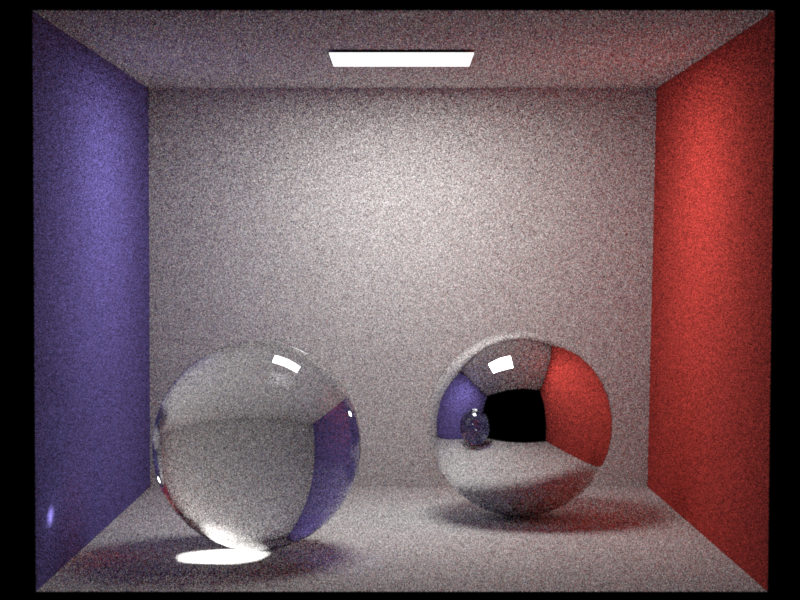
\includegraphics[width=.6\linewidth]{images/cbox_path_512.png}
\caption{Imagen generada utilizando \textit{Path Tracing} simple (512 muestras)}
\label{fig:disp}
\end{figure}

Como puede verse en la imagen se han conseguido varios efectos de iluminación global, como son los reflejos en la esfera de espejo o la cáustica en la esfera que representa un cristal, además de un ligero \textit{color bleeding} en el techo proveniente de las paredes. Sin embargo, se aprecia una gran cantidad de ruido tanto en las paredes como en los reflejos, teniendo en cuenta la gran cantidad de muestras utilizadas (512).\\

Por otro lado, la convergencia de la imagen no es muy buena debido a que solamente los caminos que intersequen con una fuente de luz contribuirán a la iluminación final. Por lo tanto, una gran cantidad de muestras se desperdician al no encontrar la luz.

\subsection{Path Tracing with Next-Event Estimation}
En esta parte de la práctica se va a implementar un \textit{Path tracer} algo más sofisticado que resuelva algunos de los problemas de la versión anterior. En concreto, trata de resolver el problema de convergencia que provocan los caminos que no intersecan con ninguna luz y que, por tanto, no aportan nada a la escena. Para resolver esto se va a calcular en cada rebote la iluminación directa que recibe ese punto desde una fuente de luz, consiguiendo con ello que cada rebote tenga, en la mayoría de los casos, un mínimo de aporte de luz garantizado haciendo que todos los rebotes contribuyan a la iluminación, lo que mejora la convergencia. Además se siguen trazando los rayos impuestos por la BRDF para conservar la iluminación global.\\

Para realizar esta tarea se ha partido del código implementado en la sección anterior, pero se ha añadido un nuevo bloque de código que para cada rebote muestrea una fuente de luz aleatoria y calcula su aportación a la luz del punto a tratar como:
$$ L += \frac{Li * brdf_{nee} * V * W}{pdf_{dir} * pdf_{light}}$$

Donde $Li$ es la iluminación directa que llega al punto desde la fuente de luz muestreada; $brdf_{nee}$ es el término BRDF teniendo en cuenta las direcciones del rayo de entrada y del rayo de salida (el que va hacia la luz); $V$ es el termino de visibilidad, ya que como hemos muestreado la luz esta podría estar ocluida; y por último, $pdf_{light}$ y $pdf_{dir}$ son las PDF de la luz muestreada y del punto en concreto muestreado, respectivamente. \\

Adicionalmente hay que tener en cuenta que al incluir un rayo directo a la luz puede darse el caso de que para un mismo punto se sume la aportación de una fuente de luz dos veces, una al muerstrear esa fuente de luz y la otra si el rayo de la BRDF interseca con esa misma fuente de luz. Para evitar estos casos se ha añadido un \textit{flag} que indica si se debe contar la iluminación si la BRDF cae en una fuente de luz o no, mientras que la aportación de \textit{Nee} siempre se tiene en cuenta. Debiendo contar con la iluminación de la BRDF si es el primer rebote, para evitar que las fuentes de luz se vean negras o si el material es completamente especular, es decir, de tipo \textit{EDISCRETE}, ya que este tipo de materiales no pueden muestrearse utilizando iluminación directa (tanto su BRDF como PDF devuelven siempre 0).\\

\begin{figure}[h]
\centering
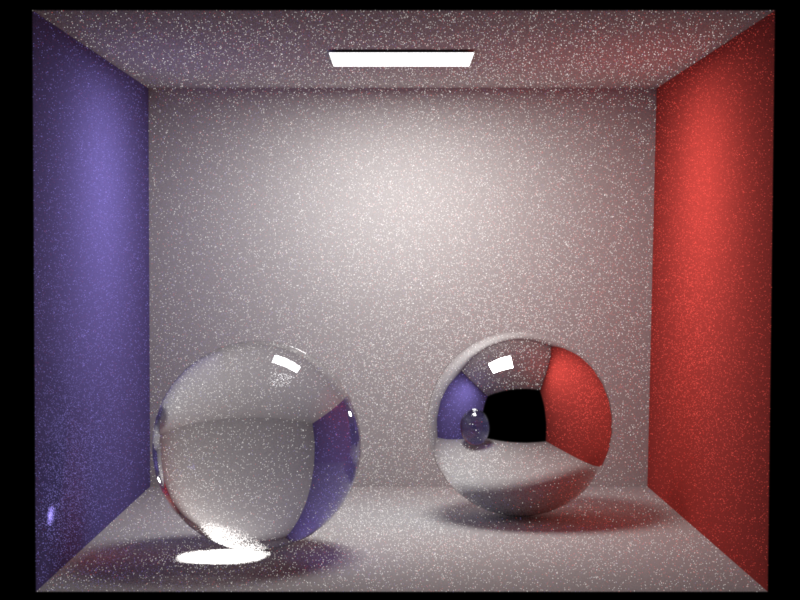
\includegraphics[width=.6\linewidth]{images/cbox_pathNee_128.png}
\caption{Imagen generada utilizando \textit{Path Tracing} con \textit{Nee} (128 muestras)}
\label{fig:disp}
\end{figure}

Como puede observarse en la imagen, se ha conseguido el resultado esperado obteniendo muchísima mejor convergencia con un numero mucho inferior de muestas para esta escena, donde ha mejorado tanto la iluminación de las paredes como los reflejos . Sin embargo, sigue existiendo ruido de alta frecuencia introducido por los rebotes especulares y las refracciones de los materiales que este metodo no elimina, pero podrian reducirse implementando \textit{Multiple Importance Sampling}.\\
 
 \subsection{Interesting Image}
En esta imagen de ejemplo se pueden observar la mayoría de efectos que se peuden conseguir utilizando \textit{Path Tracing} con \textit{Next-Event Estimation} utilizando nuestra implementación.

\begin{figure}[h]
\centering
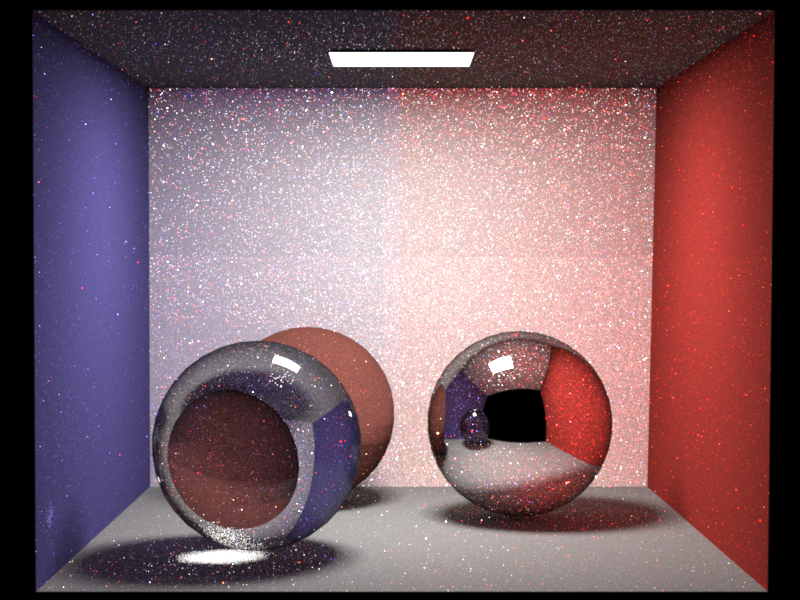
\includegraphics[width=.6\linewidth]{images/cbox_interesting_nee_512.png}
\caption{Imagen generada utilizando \textit{Path Tracing} con \textit{Nee} y un valor bajo de absorción}
\label{fig:disp}
\end{figure}

Para la generación de esta imagen se ha utilizado un nivel más bajo de absorción (modelado por la probabilidad de sobrevivir a la ruleta rusa), para conseguir que la esfera del dieléctrico se viera más clara y además la cáustica fuese más acentuada. Sin embargo, al bajar la absorción nos encontramos con un exceso de \textit{color bleeding} en la pared del fondo. Esto se debe a que en nuestra implementación se utiliza la misma probabilidad de sobrevivir a un rebote para todos los materiales de la escena. En la realidad no ocurre así y cada material tienen un nivel de absorción distinto. Por ejemplo, el nivel de absorción del cristal sería muy inferior al de las paredes y, por tanto, si obtuviésemos la probabilidad de sobrevivir a un rebote del material en cuestión, en lugar de una constante global, se podrían conseguir escenas más realistas pudiendo eliminar el \textit{color bleeding} sin oscurecer las esferas.

\end{document}
